Our project consists of two distinct programs.
One to generate the terrain and one to visualize it.

\subsection{Generation}

The generation program will feature a simple graphical user interface to change the generator parameters.
This allows the user to control the output of the program.
See Figure~\ref{fig:gui-mockup} for a mockup of the GUI.

\begin{figure}[H]
	\centering
	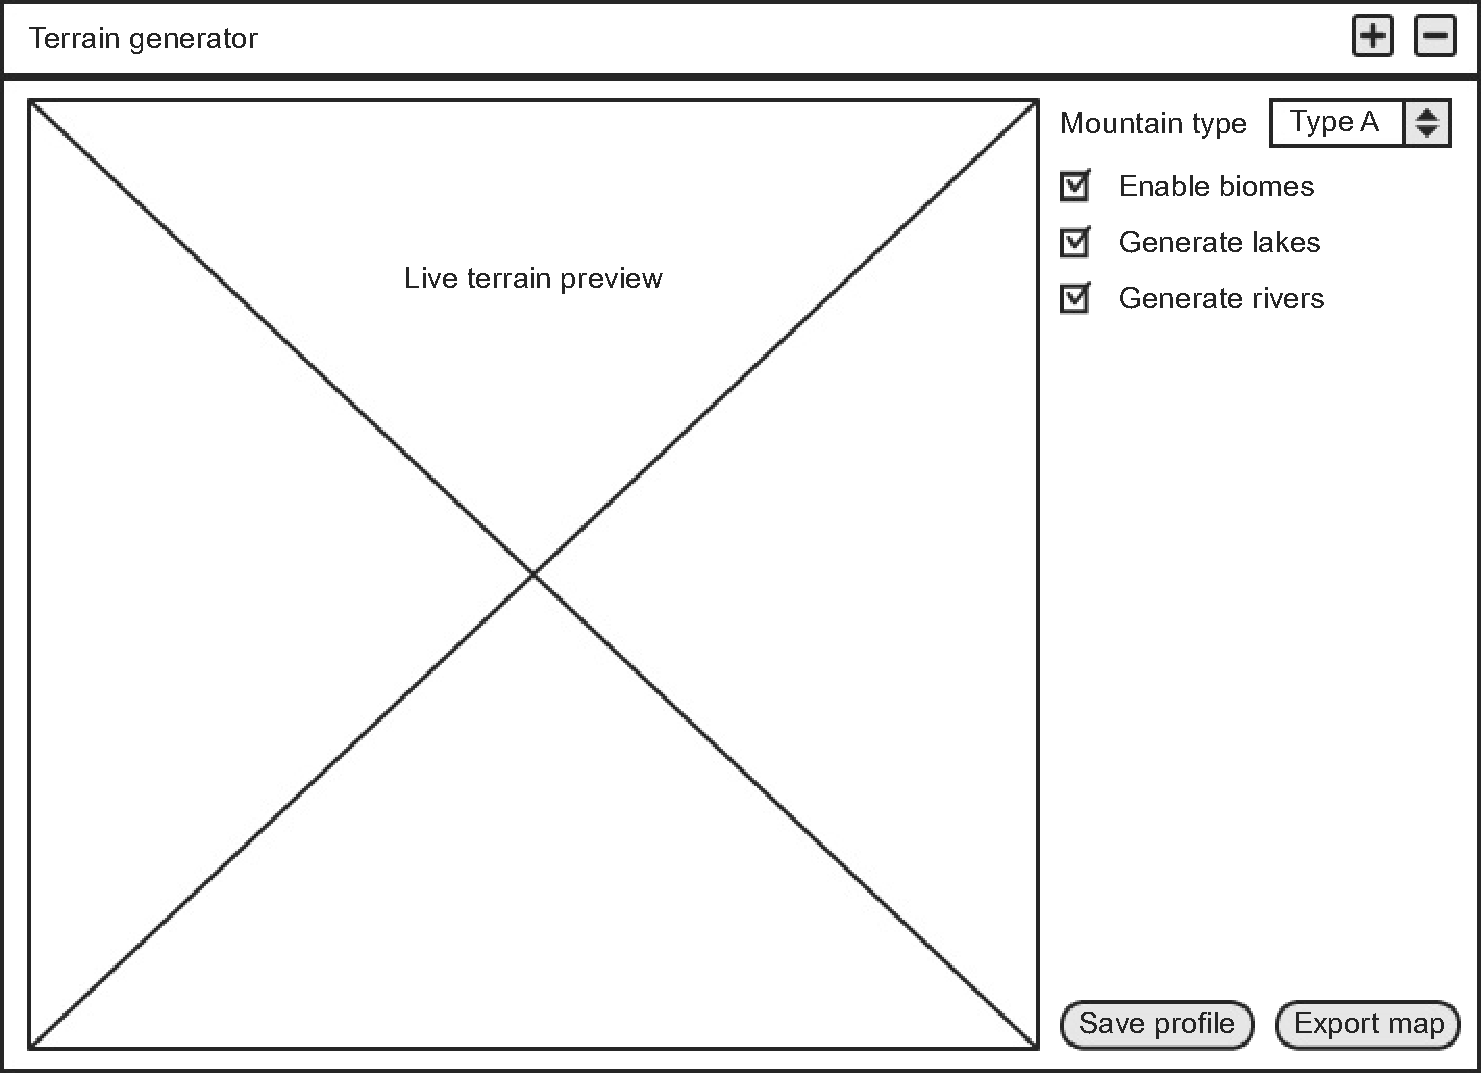
\includegraphics[width=\linewidth]{generator-gui}
	\caption{Mockup of the generator GUI}
	\label{fig:gui-mockup}
\end{figure}

The program will also feature a very simple preview of the terrain, and a button to export the terrain as a file.
This file will contain all info needed to visualize the terrain, and can be read by the visualisation program.

\subsection{Visualisation}

The visualisation program will feature a 3D view through which the user can look at the world.

The user will be able to move through and explore the map in first person view.
This can be done either walking, with the viewport height fixed to the elevation of the terrain or flying to allow for a better overview of the entire landscape.

Depending on time constraints, we will add some more challenging modes of transportation, such as swimming or using vehicles.

